\documentclass[10pt, a4paper]{article}

\usepackage[margin=2.5cm]{geometry}
\usepackage[utf8]{inputenc}
\usepackage[danish]{babel}
\usepackage{amsmath}
\usepackage{graphicx}
\usepackage{subfig}
\usepackage{listings}
\usepackage{tikz}
\usepackage{fancyvrb}
\usepackage{hyperref}

\renewcommand{\FancyVerbSpace}{\textcolor{lightgray}{.}}

\usetikzlibrary{calc}

\lstset{
  numbers=left,
  numberstyle=\tiny\color{gray},
  basicstyle=\small\ttfamily,
  aboveskip=0pt,
  belowskip=0pt
}

\title{\textsc{\Huge Maze Runner}\\\textsc{Programmeringskonkurrence}}
\date{}
\author{{\small Forfattere:
    Mads Okholm Bjørn,
    Andreas Halkjær From,
    Marcus Skov Hansen,
    Martin Hemmingsen,
  }\\{\small
    Thomas Søren Henney,
    Johan Bloch Madsen,
    Marcus Pagh,
    Tord Joakim Stordalen
}}

\begin{document}

\maketitle

\section{Introduktion}
Formålet med denne konkurrence er at designe og implementere et program, der kan føre robotter gennem en dynamisk labyrint.
De indsendte programmer bliver sat til at dyste mod hinanden, og gruppen, der har lavet det bedste program vinder selvfølgelig en præmie!

Man kan deltage i konkurrencen i grupper bestående af op til fire studerende, og deltagelse tæller som en bestået skriftlig obligatorisk afleveringsopgave for alle gruppemedlemmer.
Der skal ikke skrives nogen rapport.
Flere praktiske informationer findes sidst i dette dokument.
Bemærk dog følgende vigtige datoer:

\begin{description}
\item [20. april] Deadline for at aflevere som mandatory på CodeJudge.
\item [27. april] Deadline for at deltage i konkurrencen på CodeJudge.
\item [4. maj] Præmieoverrækkelse. Resultatet af konkurrencen præsenteres og vinderne annonceres.\\Sted: 116/81.
\end{description}

\subsection{Kort om labyrinten}
I Maze Runner gælder det om at give instruktioner til robotter, så de bevæger sig rundt på en forudbestemt bane, så en hvilken som helst robot når en bestemt position i labyrinten.
En robot kan på et træk bevæge sig enten op, ned, til venstre eller til højre, dog ikke ind i labyrintens vægge, andre robotter eller ud af banen.
Det gælder om at få en robot til at ende på målfeltet med færrest mulige samlede træk, altså inklusive træk med eventuelle andre robotter.
For at opnå en løsning med få træk, er det meget ofte en fordel (og nogle gange også nødvendigt) at flytte på mere end en robot.

I labyrinten findes også to slags kontakter der tænder og slukker for stykker af labyrintens mure.
Begge slags kontakter aktiveres ved at en robot stiller sig på dem.
Den første slags, kaldet skift-kontakter, har fortsat effekt efter robotten flytter sig til et andet felt.
Den anden slags, kaldet stå-kontakter, slukker kun for et stykke mur mens en robot står på den.

Hvis et felt er frit i tidsskridt $t$ og en robot står ved siden af feltet, kan den flytte sig så den står på feltet i tidsskridt $t+1$.
Dette gælder også selvom robotten f.eks. står på den kontakt der gør feltet frit.

\newsavebox{\simpleboard}
\begin{lrbox}\simpleboard%
\hspace{1cm}
\begin{minipage}[b]{2.1cm}%
\begin{Verbatim}[frame=single, numbers=left, showspaces, commandchars=\\\{\}, baselinestretch=0.64]
10 6
2
2 1
         0\phantom{}
   ###   B\phantom{}
#  #!#1   \phantom{}
   ###    \phantom{}
 # #      \phantom{}
 A      #a\phantom{}
A 0 2
B 5 2
a 8 5
\end{Verbatim}
\end{minipage} 
\hspace{1cm}
\end{lrbox}

\newsavebox{\simpleboardsolution}
\begin{lrbox}\simpleboardsolution%
\hspace{1cm}
\begin{minipage}[b]{2.1cm}%
\begin{Verbatim}[frame=single, numbers=left,showspaces, commandchars=\\\{\}, baselinestretch=0.64, label={\scriptsize Løsning 1}]
1R
1R
1R
1U
1D
1L
1L
1L
1L
1L
\end{Verbatim}
\vspace{-4pt}
\begin{Verbatim}[frame=single, numbers=left,showspaces, commandchars=\\\{\}, baselinestretch=0.64, label={\scriptsize Løsning 2}]
0D
1L
1L
\end{Verbatim}
\end{minipage}
\hspace{1cm}
\end{lrbox}

\begin{figure}
\centering
\subfloat[Eksempel på en bane. De grå prikker er mellemrum.\label{fig:simpleboardfile}]{
\usebox\simpleboard
}
\hspace{0.2cm}
\subfloat[Visualisering af banen til venstre.\label{fig:simpleboardgui}]{
\begin{minipage}[b]{5cm}
  \centering
  \begingroup\fboxsep=0pt
  \fbox{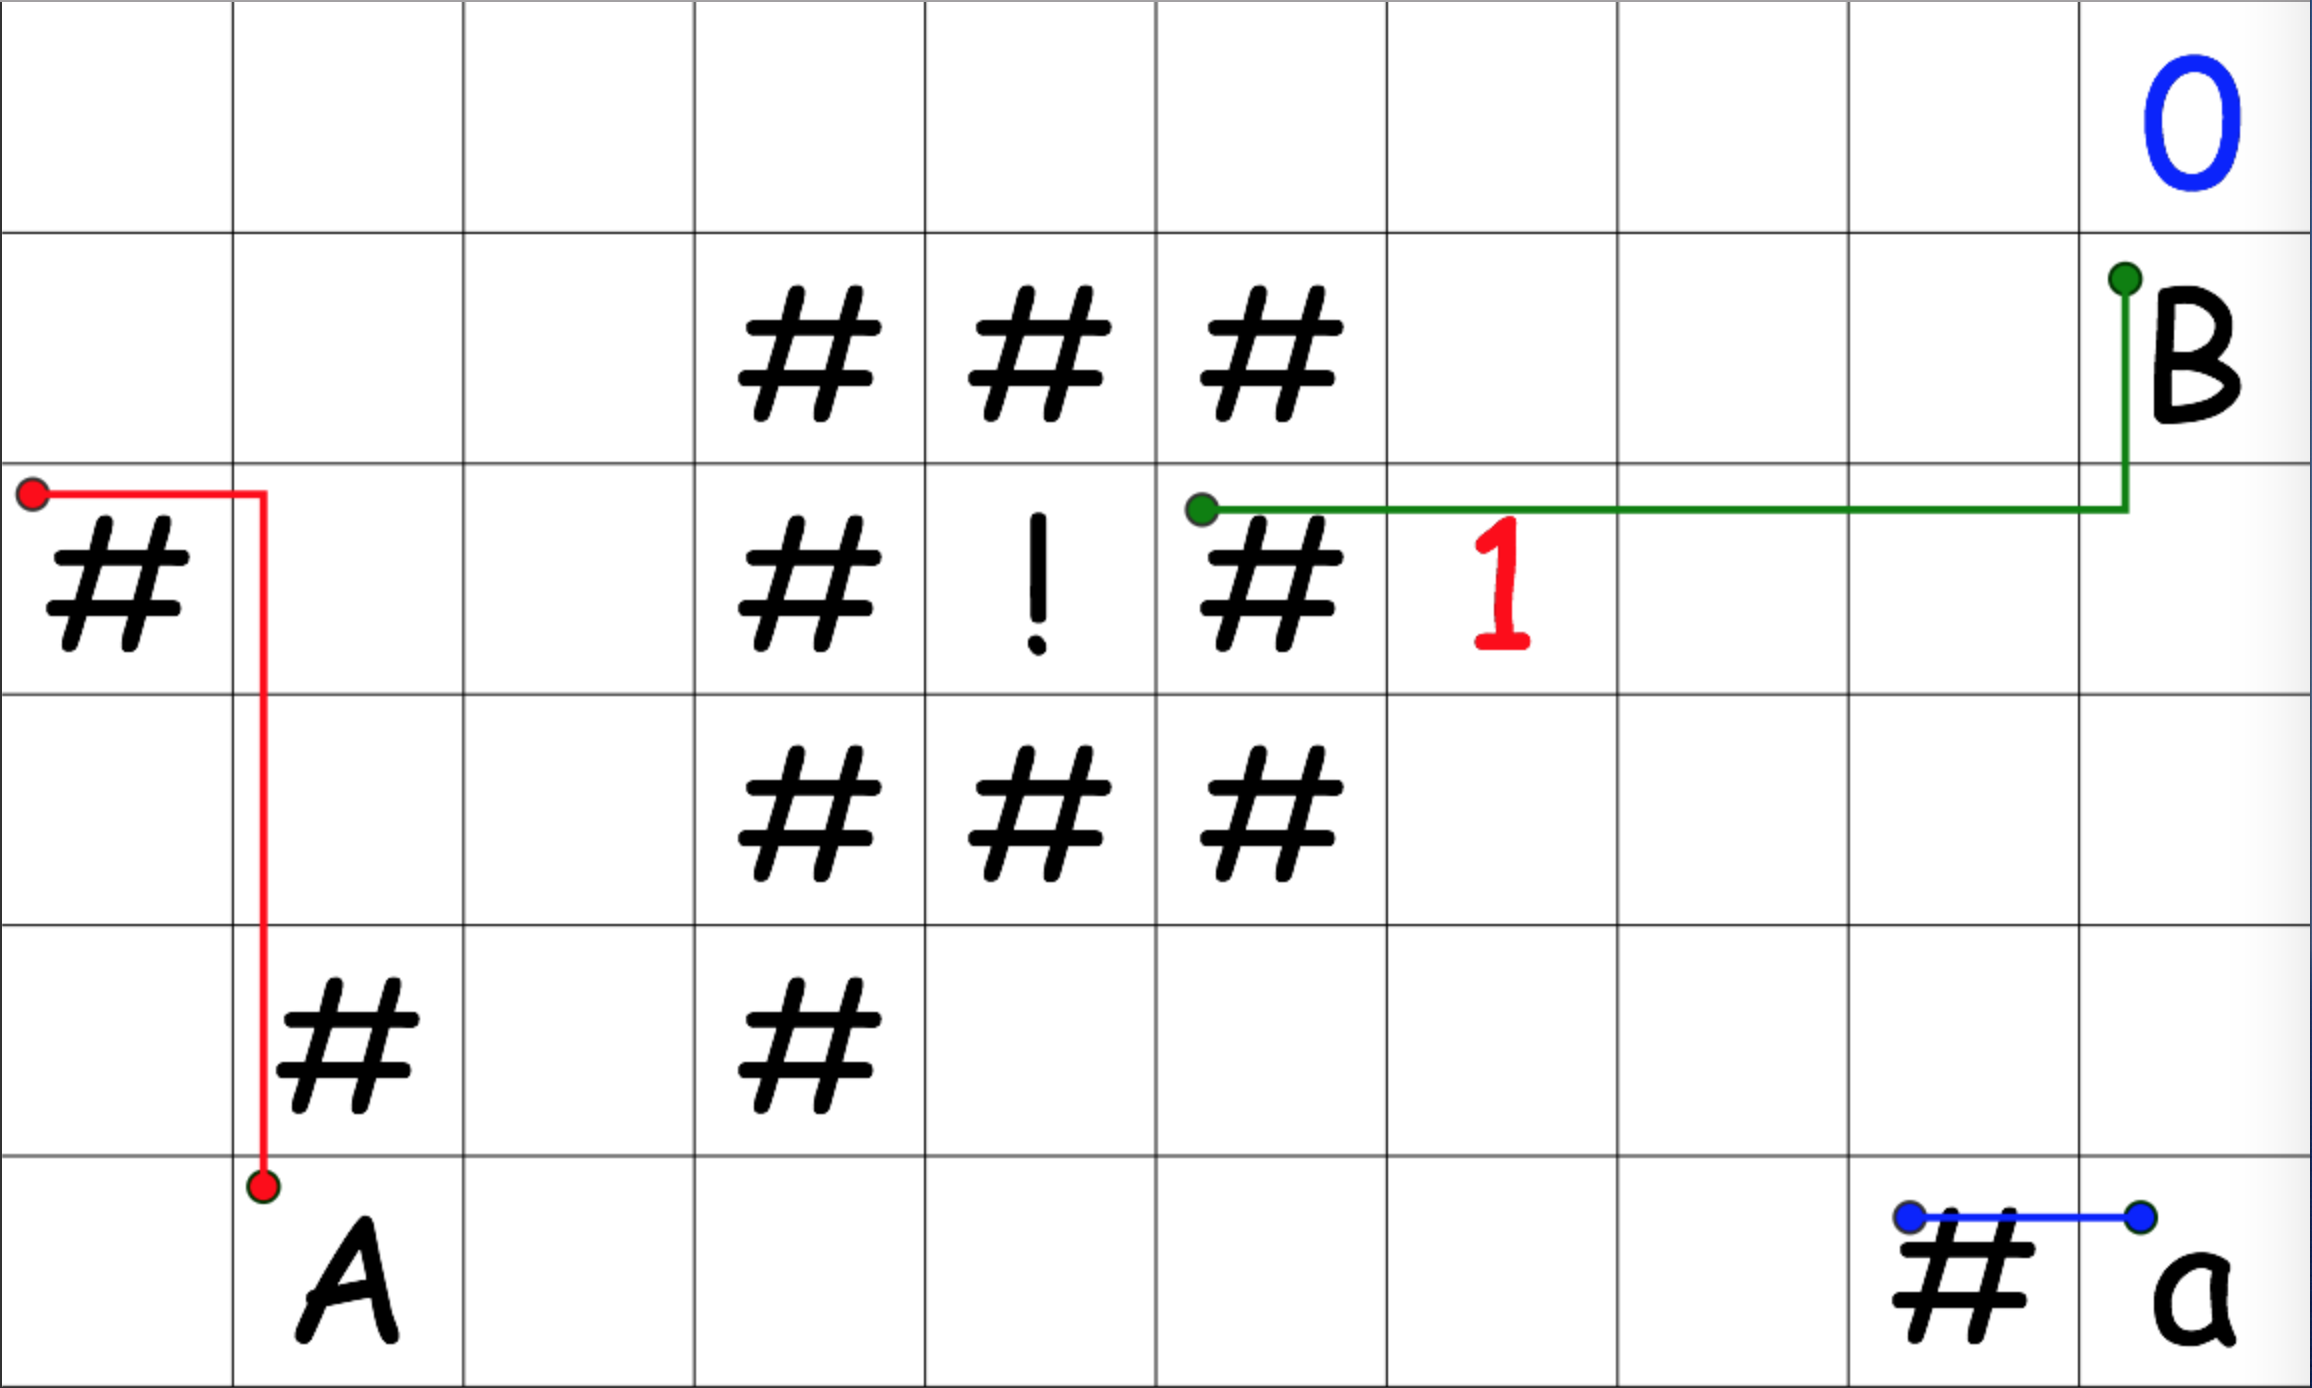
\includegraphics[height=3cm]{img/simpleboard.png}}
  \endgroup
\end{minipage}
}
\hspace{0.2cm}
\subfloat[To gyldige løsninger af henholdsvis længde 10 og 3.\label{fig:simpleboardsolutions}]{
  \usebox\simpleboardsolution
}
\caption{Eksempel på en bane af størrelse $n=10$ med $r=2$ robotter. De sorte felter er vægge, og det grønne felt er målfeltet for robotterne. Den optimale løsning til denne bane har længde 3.}
\label{fig:simpleboardexample}
\end{figure}

\section{Konkurrencen}
I konkurrencen vil vi arbejde med en tekst-baseret repræsentation af labyrinten.
Labyrinten ligger på et rektangulært gitter (kaldet banen) bestående af $n$ søjler og $m$ rækker, hvor $2 \leq n,m \leq 1000$.
I banen findes $r$ robotter, hvor $1 \leq r \leq 10$. Robotterne er nummeret $0, \ldots, r-1$, og det gælder blot om at få en af robotterne hen på det unikke målfelt.

Figur~\ref{fig:simpleboardexample} viser et eksempel på en bane med $n=10, m=6$ og $r=2$ samt to mulige løsninger. I de næste to sektioner beskrives det formelle input- og outputformat samt kravene til jeres program.

\subsection{Inputformat}
Inputtet til jeres program er en bane som vist i Figur~\ref{fig:simpleboardfile}.

Den første linje angiver henholdsvis bredden,  $n$, og højden, $m$,  af banen som to mellemrumsadskilte heltal mellem $2$ og $1000$.
Den anden linje angiver antallet af robotter, $r$, som et heltal mellem $1$ og $10$.
Den tredje linje angiver antallet af skift-kontakter, $\Lambda$, og stå-kontakter, $\lambda$, som to heltal mellem $0$ og $26$ adskilt af mellemrum.

De efterfølgende $m$ linjer angiver banen.
Hver af disse linjer består af $n$ symboler, der repræsenterer indholdet på denne position i banen.

De lovlige symboler i en linje er:

\begin{description}
\item[\texttt{\#}]: Angiver at positionen er en væg.
\item[(mellemrum)]: Angiver at positionen er tom.
\item[\texttt{!}]: Angiver målpositionen.
\item[\texttt{0, 1}, \ldots, $(r-1)$]: Angiver, at robotten med dette tal er på denne position.
\item[\texttt{A, B, \ldots, Z}]: Angiver skift-kontakter.
\item[\texttt{a, b, \ldots, z}]: Angiver stå-kontakter.
\end{description}

Det garanteres, at symbolet \texttt{!}, robotterne \texttt{0, 1}, $\ldots (r-1)$ og kontakterne $a-z$ og $A-Z$ optræder på præcis én position i banen.
Det garanteres desuden at banen kan løses.

De resterende $\Lambda+\lambda$ linjer består af navnet på en kontakt og dernæst koordinaterne for det felt, som kontakten påvirker, se figur \ref{fig:simpleboardfile}.
Der vil altid initielt være en mur på det givne felt.
Alle skift-kontakter angives først, dernæst alle stå-kontakter.
Koordinaterne er givet som 0-indekserede par af søjler henholdsvis rækker, så eksempelvis har robot 1 på figur \ref{fig:simpleboardfile} koordinaterne $2, 6$.
To kontakter kan ikke påvirke den samme mur.
Hvis en robot står på et felt, hvor der dukker en mur op, ender robotten oven på muren.
Herfra kan robotten dog kun bevæge sig ned på et ledigt felt.

\subsection{Outputformat}
En gyldig løsning til banen er en sekvens af træk, der bringer en robot hen på målpositionen.
Hvert træk udskrives som en linje bestående af præcis to symboler: Et heltal $i$ der angiver robotten, hvor $0 \leq i \leq r-1$, efterfulgt (uden mellemrum) af et af symbolerne \texttt{R} (højre), \texttt{L} (venstre), \texttt{U} (op) eller \texttt{D} (ned) der angiver retningen.
F.eks. angiver \texttt{0R} at robot 0 flyttes mod højre. Et eksempel på to gyldige løsninger er vist i Figur~\ref{fig:simpleboardsolutions}.

\subsection{Krav til jeres program}
Jeres program skal indlæse en bane fra konsollen (\texttt{stdin}), beregne en gyldig løsning og udskrive denne løsning til konsollen (\texttt{stdout}).
Det er ikke et krav at jeres program finder den korteste løsning, men jo kortere løsningen er, desto flere points får jeres program.

\section{Sådan kommer du igang -- og anden praktisk information}
Start med at hente filen \texttt{mr.zip}, der ligger på CodeJudge under \texttt{Assignments} $\Rightarrow$ \texttt{Programming Competition (Maze Runner)} $\Rightarrow$ \texttt{Mandatory}.
Filen indeholder en skabelon i hhv. Java og Python med forskellige brugbare metoder til indlæsning af banefiler m.m.
Prøv at uploade filen \texttt{MazeRunner.java} til CodeJudge -- så burde den klare den første test.

Det er ikke et krav at tage udgangspunkt i disse skabeloner -- I må også meget gerne skrive jeres løsning i andre sprog, der er understøttet på CodeJudge.

Filen \texttt{mr.zip} indeholder desuden en række forskellige baner, som I kan teste jeres løsning på.
Alle banefilnavne starter med et tal, der angiver, hvor mange robotter, der er i banen.

Herunder følger yderligere relevant information.

\paragraph{Piazza} Brug Piazza til alle spørgsmål, der ikke er besvaret her.

\paragraph{Gruppedannelse} Husk at danne gruppe på CodeJudge.
Maksimum er fire studerende per gruppe.
Aflevering foregår ved at uploade sin løsning til CodeJudge.

\paragraph{CodeJudge} Konkurrencen foregår på CodeJudge og er opdelt i to delopgaver: \emph{Obligatorisk} og \emph{Konkurrence}.
Den obligatoriske del består af forholdsvis nemme baner med en enkelt robot.
Start med at lave en løsning til denne del.
Konkurrencedelen indeholder større og mere udfordrende baner med op til 10 robotter.

\paragraph{Den obligatoriske del} Uploades en løsning, der består alle tests (5 synlige og 5 skjulte) i den obligatoriske del, tæller dette som en bestået skriftlig obligatorisk afleveringsopgave for alle medlemmer af gruppen.

\paragraph{Konkurrencedelen} Efter deadline tager vi den nyeste version af jeres program i konkurrencedelen og lader det dyste mod de andre programmer på en ukendt samling af baner.

\paragraph{Tids- og hukommelsesgrænser} På CodeJudge bliver jeres program tildelt $T$ sekunders CPU-tid og $S$ MB hukommelse. I kan læse værdierne $T$ og $S$ som de første to kommandolinjeargumenter til jeres program. Som udgangspunkt kan I regne med at $T=5$ sekunder og $S=500$MB, men når den endelige konkurrence afvikles efter deadline, bliver jeres program tildelt en del flere ressourcer.

\paragraph{Pointtildeling} For hver bane i konkurrencedelen som jeres program løser får det $100 \frac{E}{U}$ points, hvor $U$ er længden af jeres løsning, og $E$ er et estimat af den bedst mulige løsning for banen.

\paragraph{Scoreboard} På Scoreboardet på CodeJudge kan man løbende følge med i, hvordan ens løsning klarer sig i forhold til andre gruppers løsninger.
Grupperne er sorteret efter det totale antal points deres løsning har opnået på konkurrencebanerne.
I tilfælde af point-lighed er den bedste gruppe den med det korteste tidsforbrug.
Bemærk, at vi til den endelige konkurrence også tester jeres program på nye og ukendte baner, så derfor er det ikke sikkert, at den endelige vinder bliver den gruppe, der ligger øverst på Scoreboardet.

\noindent Hvis der er problemer med CodeJudge så kontakt Thomas.

\paragraph{Webapp} På hjemmesiden \url{https://319.dk/MR/} findes en app, hvor man kan importere/eksportere baner og løsninger -- og selv prøve at spille banen vha. tastaturet. Man kan også komme direkte til denne app ved at klikke på visualiseringen af en bane i CodeJudge. Appen er kun testet i Chrome og Safari, men burde også virke i andre browsere og på tablets og touchenheder. Bugs kan mailes til Mads Bjørn.

\paragraph{Nogle gode råd} Start med at lave en løsning, der virker for helt små baner, hvor der kun er en robot. Overvej, hvordan du kan bruge algoritmiske redskaber fra kurset som fx bredde-først-søgning og hashing til at søge efter en løsning.

\end{document}
